\begin{appendices}
	\chapter{Syllable classification through histogram segmentation} \label{appendix:split_syllables}
	
	% split audio files into three separate files (one for each syllable)
	Since the recordings are very consistent in loudness and are noise free, we can split up the files per syllable, obtaining three files per original sound (one for each syllable).
	
	A sliding window is used of size 0.02 seconds. With a sample rate of 22050, this corresponds to roughly 500 samples per window. The maximum is computed for each window. Speech signals can then be split up when a severe dip happens in the signal. Regions where the amplitude is greater than 0.2 are considered \textbf{klinkers}, the regions with with lower values are considered \textbf{medeklinkers}. Apart from a few edge cases, this technique worked well enough for this purpose. In those cases, the splitting points closest to the one-third and two-third splitting points were considered.
	
	\textbf{ERR: OUDE AFBEELDINGEN ZIJN WEG}
	%\begin{figure}[h]
	%	\centering
	%	\includegraphics[width=0.7\linewidth]{"../../../../../../../../../GitHub/thesis-fabian-denoodt/GIM/datasets/gigabo/split up graphs/test/bababa_1"}
	%	\caption{}
	%	\label{fig:bababa1}
	%\end{figure}
	%
	%\begin{figure}[h]
	%	\centering
	%	\includegraphics[width=0.7\linewidth]{"../../../../../../../../../GitHub/thesis-fabian-denoodt/GIM/datasets/gigabo/split up graphs/test/bababa_1_split"}
	%	\caption{}
	%	\label{fig:bababa1split}
	%\end{figure}
	
	
	
	note: we do need a hard threshold which is based on the signal's intentisity level. One could consider the alternative approach of looking at the gradient at each point and selecting the points with largest negative gradient. This will work in many cases, however, not for temporal envelops which gradually move towards zero, s.t: \ref{fig:example where gardient doesnt work}. Instead we use a dynamic threshold. This threshold is computed by creating transforming the signal into bins of 90'th percentile, creating a histogram of the single signal and applying otsu's image segmentation algorithm to obtain the threshold of that single audio sample.
	We also tried directly applying otsu to the moving average and maximum of the bins. This either gave a threshold that was too small or too large. the 90th percent resulted in an acceptable compromise.
	
	
	\begin{figure}[h]
		\centering
		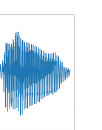
\includegraphics[width=0.7\linewidth]{screenshot011}
		\caption{}
		\label{fig:example where gardient doesnt work}
	\end{figure}
	
	
	
	Example where the explained strategy does not work: %\ref{fig:badadi1}
	%\begin{figure}[h]
	%	\centering
	%	\includegraphics[width=0.7\linewidth]{"../../../../../../../../../GitHub/thesis-fabian-denoodt/GIM/datasets/gigabo/split up graphs/train/badadi_1"}
	%	\caption{}
	%	\label{fig:badadi1}
	%\end{figure}/
	
	Reference images for in the text:
	\begin{figure}
		\centering
		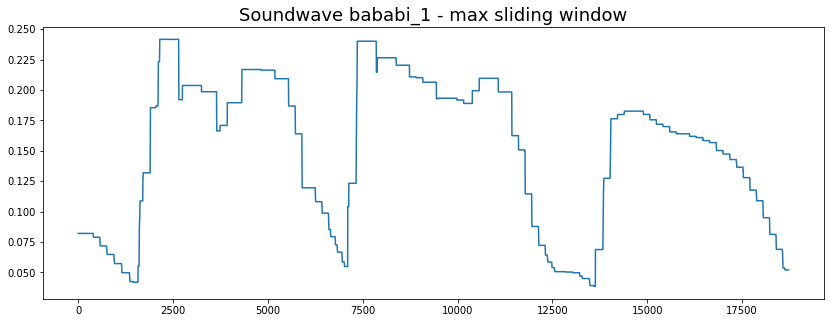
\includegraphics[width=0.7\linewidth]{screenshot012}
		\caption{}
		\label{fig:max sliding window}
	\end{figure}
	
	\begin{figure}
		\centering
		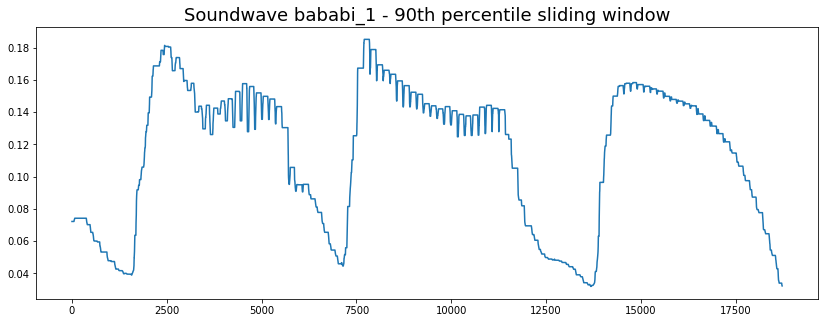
\includegraphics[width=0.7\linewidth]{screenshot013}
		\caption{}
		\label{fig:90th percentile}
	\end{figure}
	
	\begin{figure}
		\centering
		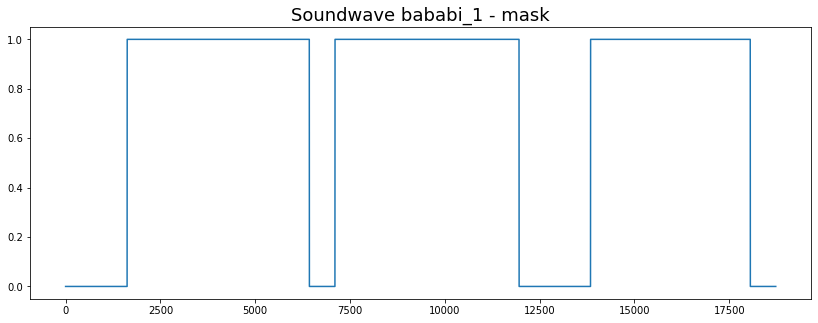
\includegraphics[width=0.7\linewidth]{screenshot014}
		\caption{}
		\label{fig:mask}
	\end{figure}
	
	\begin{figure}
		\centering
		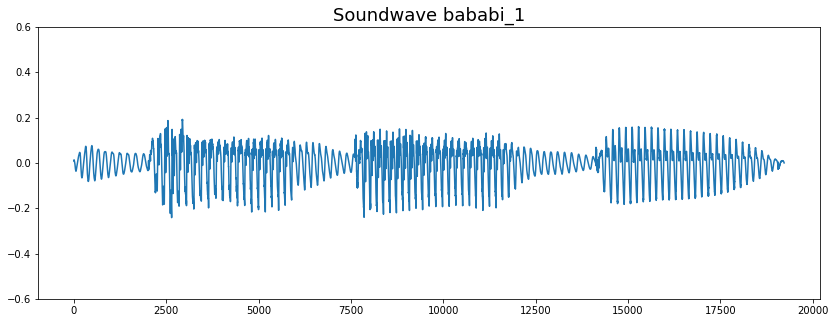
\includegraphics[width=0.7\linewidth]{screenshot017}
		\caption{}
		\label{fig:full sound wave adjusted yaxis}
	\end{figure}
	
	
	\begin{figure}
		\centering
		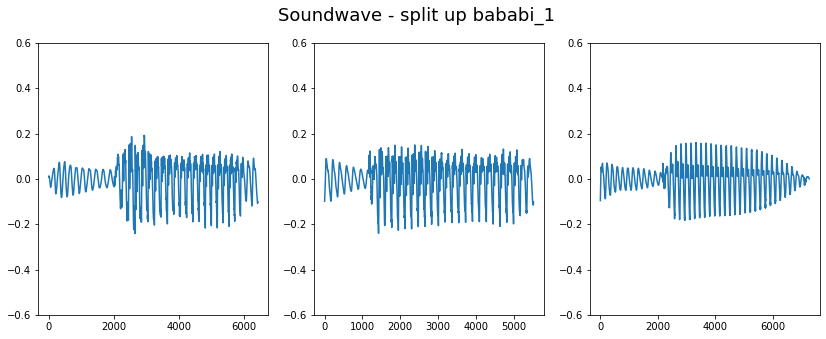
\includegraphics[width=0.7\linewidth]{screenshot016}
		\caption{}
		\label{fig:split up sound wave}
	\end{figure}
	
	
	\begin{figure}
		\centering
		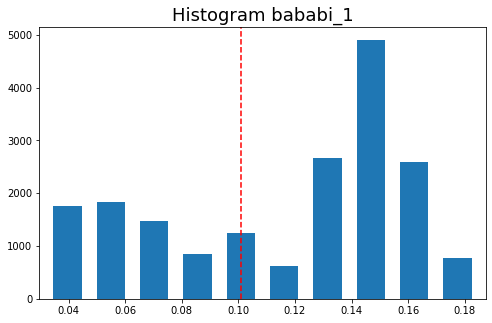
\includegraphics[width=0.4\linewidth]{screenshot018}
		\caption{}
		\label{fig:histogram}
	\end{figure}
	
	
	audio padded to maximum length. (added zeros in front and back)
	
	\chapter{Some more appendix}
	\section{GIM: Activations visualisations}
	
	%these were notes from the decoder from file: eval_autoencoder.py
	thought for later: its actually weird i was able to play enc as audio as enc is 512 x something
	so huh? that means that a lot of info is already in first channel? what do other 511 channels then contain?
	"""
	Observations:
	First layer decoded still contains the same sound, but with some added noise (could be because decoder hasn't trained very).
	However, the encoded first layer, still contains the exact sound as the original sound. It is however downsampled a lot -> from 16khz to ~3khz
	"""
	thought for later: its actually weird i was able to play enc as audio as enc is 512 x something
	so huh? that means that a lot of info is already in first channel? what do other 511 channels then contain?
	
	
	
	\begin{figure}[h]
		\centering
		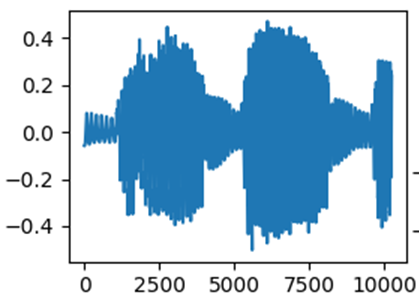
\includegraphics[width=0.7\linewidth]{screenshot007}
		\caption{"BA-BA-BA" time domain}
		\label{fig:screenshot007}
	\end{figure}
	
	\begin{figure}[h]
		\centering
		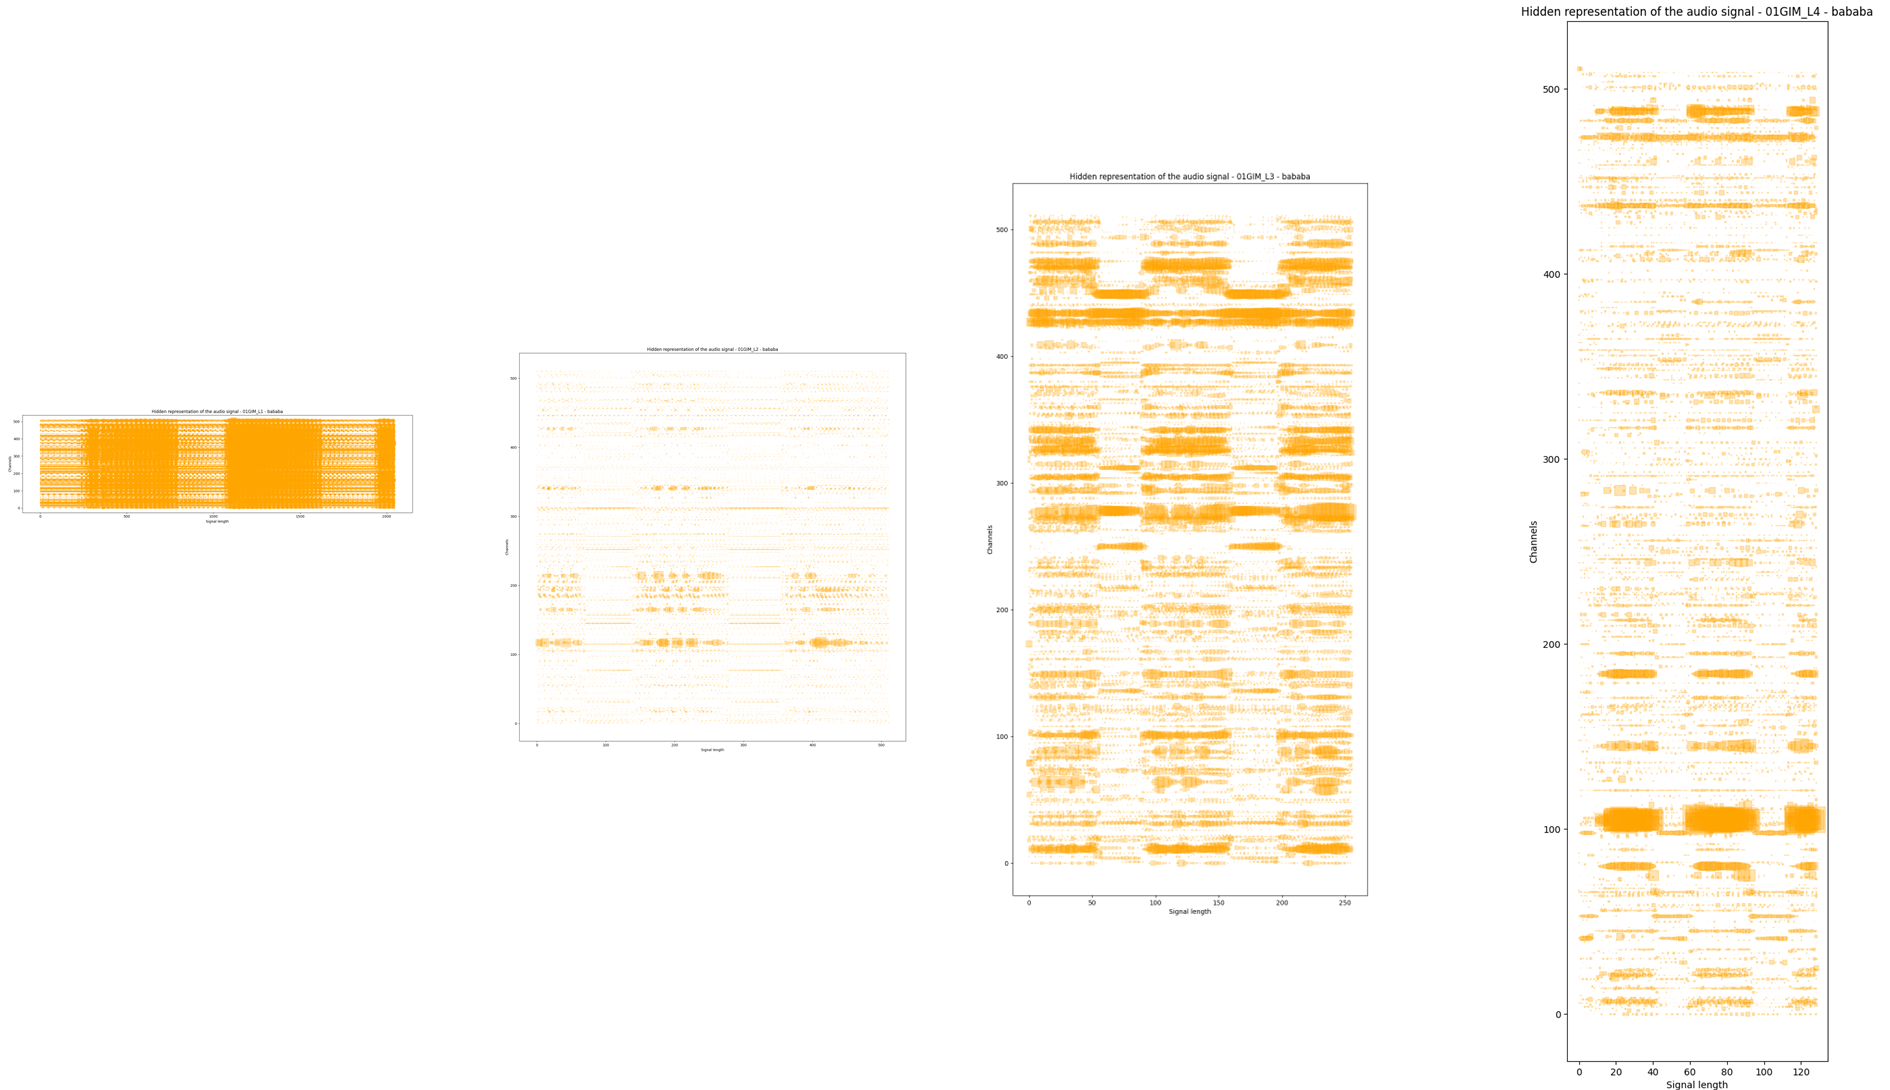
\includegraphics[width=0.7\linewidth]{screenshot006}
		\caption{Activations of the sound "BA-BA-BA" through GIM}
		\label{fig:gim latent activations}
	\end{figure}
	
	No batch normalisation, so although channels appear to have larger activations than other channels, size of activation does not really say anything about information. eg activations 0.01 could still contain more information than 3.0 activation.
	
	Since the activations from convolutional neural networks, the order is still maintained. Hence, can align activations with original signal.
	
	Observations in latent representations:
	
	\textit{Layer 1:}
	The activations of the first decoder still contain a lot of similarity with the original signal, in terms of structure. There is a lot of redundant data within the representation. Eg: the one channel could be replied 
	
	Layer 2
	
	Layer 3:
	
	Layer 4:
	Still notices multiple channels which have high activations when signal is has high amplitudes and small activations when amplitude is low. 
	
	Also activations which are high when volume is low. --> indicates that certain kernel weights are sensitive for \textbf{"klinkers"} and other kernels for \textbf{medeklinkers}. see \ref{fig:screenshot008}.
	
	\begin{figure}[h]
		\centering
		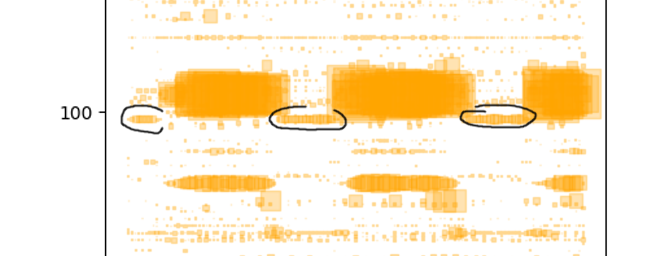
\includegraphics[width=0.7\linewidth]{screenshot008}
		\caption{zoomed in}
		\label{fig:screenshot008}
	\end{figure}
	
	
	Observe that activations happen in clusters/sequences. So it is usually a patch of signal samples that cause high activations. This could for instance indicate that both kernels are sensitive for the \textbf{medeklinker} "b", but sensitive for different features. eg the letter B has spoken sound "buh". so maybe one is sensitive for "b" and other for "uh".
	
	Figure \ref{fig:layer4 zoomed in} also nicely shows how different channels have clusters of activations at slightly different times. 
	
	\begin{figure}[h]
		\centering
		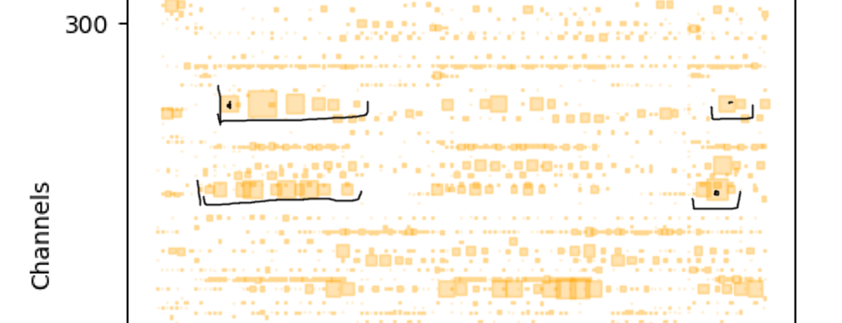
\includegraphics[width=0.7\linewidth]{screenshot010}
		\caption{Zoomed in}
		\label{fig:layer4 zoomed in}
	\end{figure}
	
\end{appendices}